Si precisa che tutti in tutti gli scenari simulati si assume che la rete sia completamente connessa per cui da un qualsiasi nodo \textit{x} è possibile raggiungere tramite uno o più nodi il nodo \textit{sink}.
\\\\
\textit{1) TX Time}: come mostrato in \textbf{Figura \ref{fig:TXTime_2}}, anche qui il tempo che in media i nodi utilizzano la wake-up Radio per trasmettere messaggi di wake-up diminuisce significativamente rispetto alla versione base di GreenWUP all'aumentare del traffico in rete. Questo è un risultato che ci si aspettava in quanto adesso i vari nodi hanno la possibilità di evitare lo scambio di pacchetti RTS/CTS con i propri vicini, che ricordiamo sono seguiti da messaggi di wake-up da e verso il nodo sender.\\
Ovviamente più pacchetti data vengono inviati e più volte si evita il classico scambio RTS/CTS, ecco perché questa variante presenta tempi in TX minori man mano che il traffico aumenta. In questo caso i miglioramenti sono tra il 50\% e il 62\%.
\\\\
\textit{2) Energy Consuption}: come mostrato in \textbf{Figura \ref{fig:EnergySpent_2}}, l'energia consumata dall'intera rete è minore rispetto l'energia consumata dalla versione base.\\
Anche in questo caso, il risultato è dovuto al fatto che ci sono molti meno scambi di RTS/CTS. In particolare questa procedura è eseguita soltanto una volta ogni quattro pacchetti data da inoltrare (dato che è possibile trasmettere verso il nodo cached per un massimo di 3 volte), inoltre, considerando che la procedura richiede l'invio di \(2 + ( 2 * n)\) pacchetti se si hanno \textit{n} possibili relay node che rispondo all' RTS del sender, è facile intuire un miglioramento nei consumi energetici di ogni nodo. I miglioramenti ottenuti sono, nel migliore dei casi (\textit{iaTime}=2), circa del 15\%. Per configurazioni con meno pacchetti si aggira invece intorno al 10-13\%.
\\\\
\textit{3) End-to-End Latency}: come mostrato in \textbf{Figura \ref{fig:Latency_2}}, non solo vi è un miglioramento rispetto la versione base di GreenWUP, ma questo fattore di miglioramento aumenta all'aumentare del traffico in rete.\\
Ovviamente questo è dovuto al fatto che in questo contesto, così come anche in altri, il concetto di \textit{caching} di informazioni dà il meglio di se in situazioni in cui il traffico è maggiore. Infatti non dovendo aspettare tempi\footnote{\'E stato citato il jitter randomico ma ovviamente ci sono anche altri tempi di attesa: ad esempio dopo l'invio di un messaggio di wake-up i nodi aspettano un tempo che permetta a chi riceve il messaggio di impostare la main radio in RX prima di mandare l'informazione.} come il jitter randomico, un nodo impiega molto meno tempo ad inoltrare un pacchetto verso un proprio vicino (se questo ovviamente è stato memorizzato in precedenza). I miglioramenti qui sono più importanti, infatti, abbiamo un miglioramento di circa il 25\% in reti molto trafficate che va a scendere fino a un minimo del 12-15\% per reti meno trafficate. 
\\\\
\textit{4) Packet Delivery Ratio}: come mostrato in \textbf{Figura \ref{fig:PDR_2}}, la percentuale di pacchetti ricevuti è paragonabile a quella della versione base, garantendo sempre la corretta ricezione di almeno il 99\% dei pacchetti.
\\\\
Ovviamente, come già detto, è molto importante per questa variante non "stressare" troppo i nodi cached in quanto se questi dovessero essere spesso non disponibili si andrebbero a fare svariate ritrasmissioni in più rispetto alla versione base, causando un degrado non sono in termini di latenza ma anche di energia consumata.\\
In questo caso, ogni nodo può trasmettere verso il nodo cached non più di 3 volte.

\begin{figure}[H]
  \begin{subfigure}[t]{0.49\linewidth}
    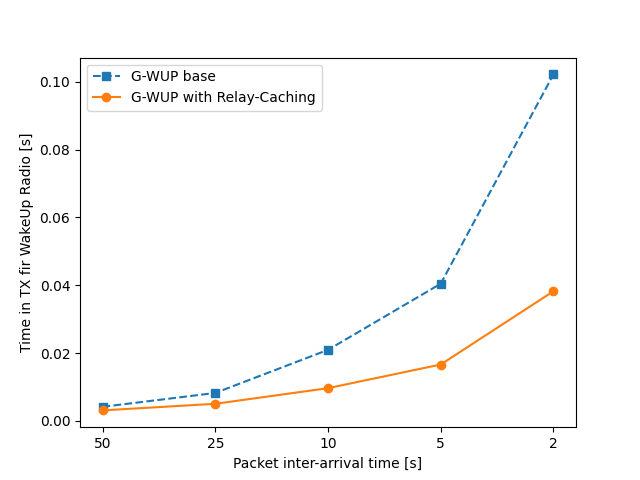
\includegraphics[width=1.1\linewidth]{Contents/Images/graphs/relayCaching/tx_time.png}
    \caption{TX Time for the WUR}
    \label{fig:TXTime_2}
  \end{subfigure}
  \begin{subfigure}[t]{0.49\linewidth}
    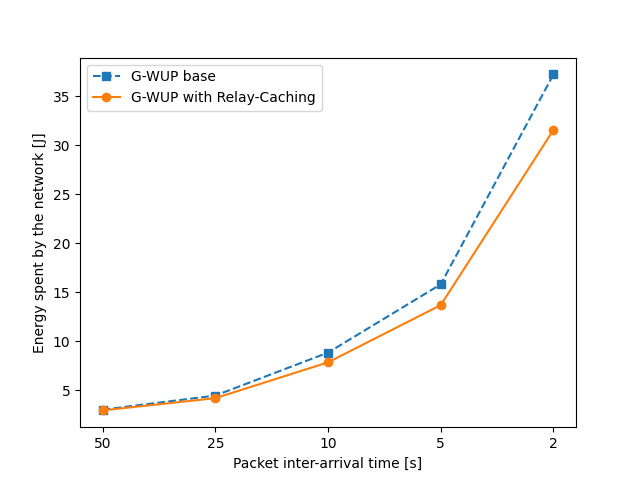
\includegraphics[width=1.1\linewidth]{Contents/Images/graphs/relayCaching/energySpent.png}
    \caption{Energy Consuption}
    \label{fig:EnergySpent_2}
  \end{subfigure}
  \begin{subfigure}[t]{0.49\linewidth}
    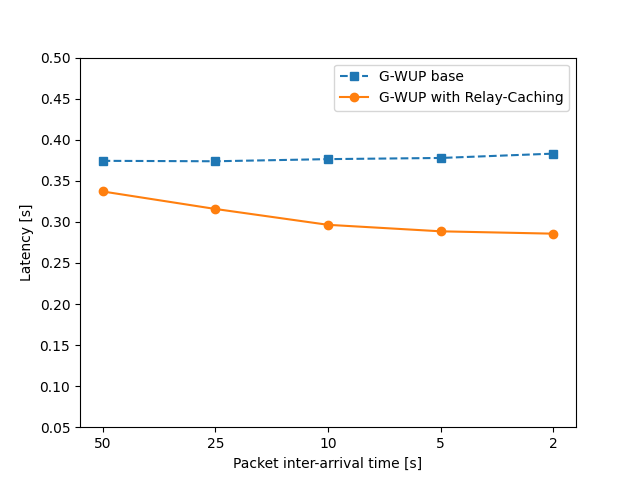
\includegraphics[width=1.1\linewidth]{Contents/Images/graphs/relayCaching/latency.png}
    \caption{End-to-End Latency}
    \label{fig:Latency_2}
  \end{subfigure}
  \begin{subfigure}[t]{0.49\linewidth}
    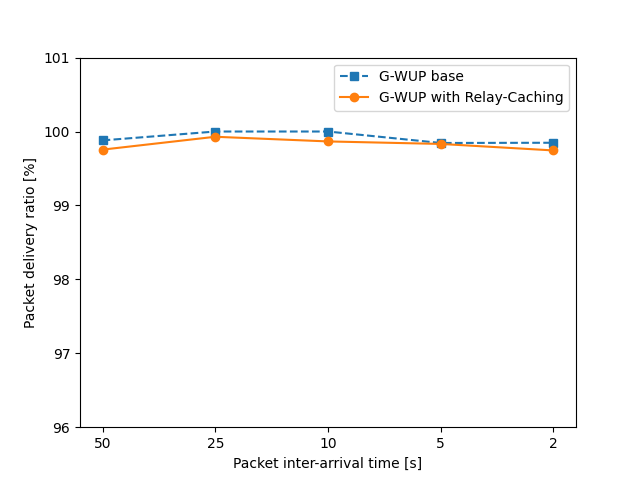
\includegraphics[width=1.1\linewidth]{Contents/Images/graphs/relayCaching/pdr.png}
    \caption{Packet Delivery Ratio}
    \label{fig:PDR_2}
  \end{subfigure}
  \caption{Confronto delle prestazioni tra versione base di GreenWUP (blu) e variante proposta (arancio)}
  \label{fig:relayCaching}
\end{figure}

In sintesi la variante che introduce il caching mostra di riuscire a ridurre significativamente il problema dell'attivazione della main radio con miglioramenti significativi in termini di energia consuma, senza degradare l'affidabilità della consegna delle informazioni. La variante riesce anche a ridurre in modo significativo le latenze, metrica importante in sistemi che, sempre piu', richiedono la rapida consegna di informazioni per supportare applicazioni "industria 4.0" o realizzare sistemi di allarme.